\chapter{模擬環境}
%\renewcommand{\baselinestretch}{10.0} %設定行距
\section{模擬模型}
 在模擬的模型上,延用了學長設計的冰球機,並進行了部分的設計變更,將原本的人機對打更改為機器對打,且因為搭配深度強化學習的訓練,所以將兩邊的擊球器都僅保留X軸向(左右)移動,而冰球則是使用原本設計。多虧了學長們所設計的冰球機模型,讓我們在運作上有問題時可以直接發問,設計變更的地方也可以快速完成。\\
\begin{figure}[hbt!]
\center
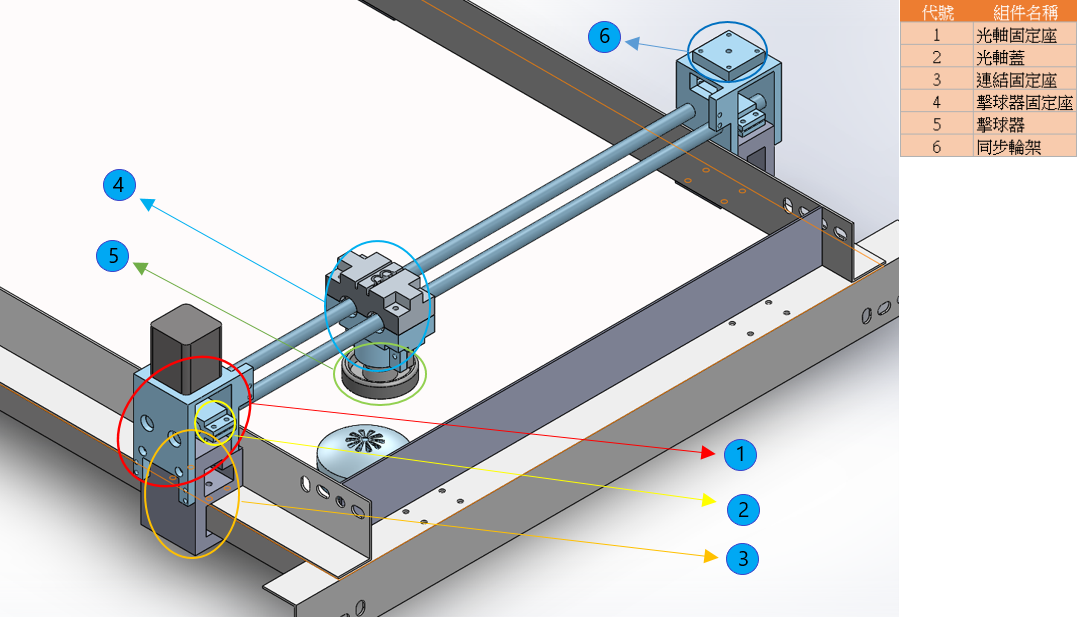
\includegraphics[width=13cm]{model}
\caption{\Large 組合圖}
\label{model}
\end{figure}

\qquad 將原本Y軸移動機構移除,並將其改為固定在特定位置上,此固定座設計是取代原本鎖在光軸固定坐上的(圖.\ref{model} 代號 1)Y軸皮帶固定座(圖.\ref{axialseat}),並使光軸固定座可以通過連結固定做鎖固於桌面,如圖.\ref{connectSeat}。\\

\begin{figure}[hbt!]
\center
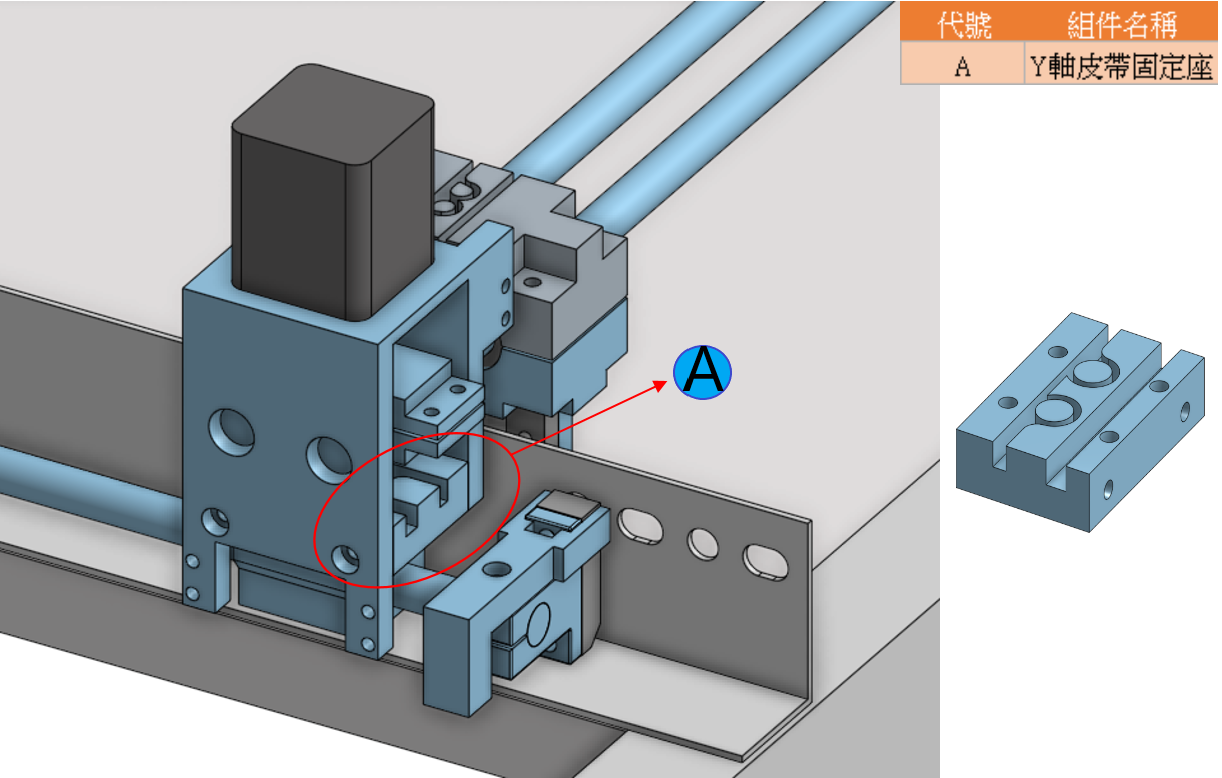
\includegraphics[width=8cm]{axialseat}
\caption{\Large Y軸皮帶固定座}
\label{axialseat}
\end{figure}

\begin{figure}[hbt!]
\center
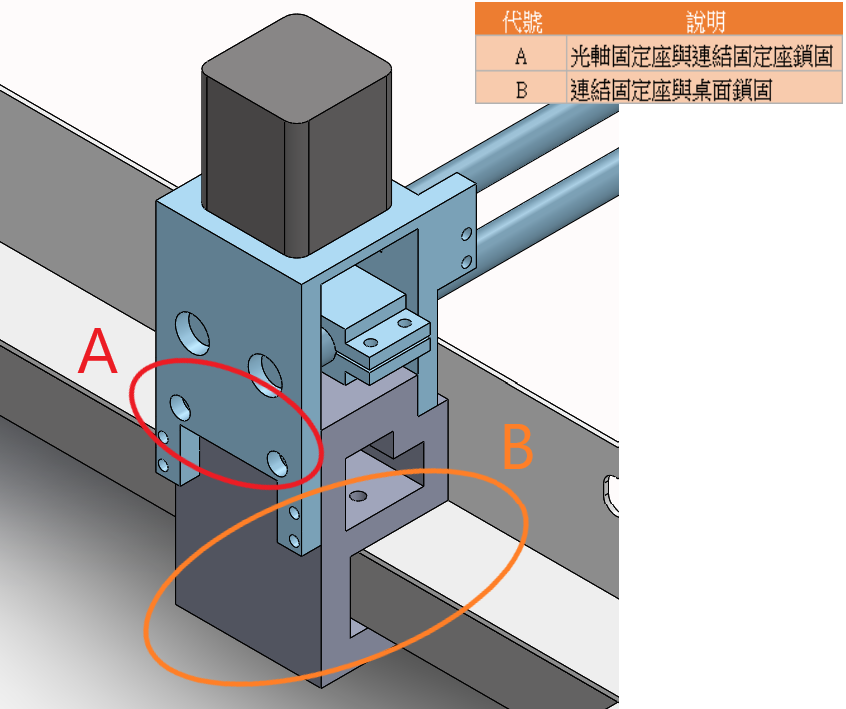
\includegraphics[width=8cm]{connectSeat}
\caption{\Large 連結固定座}
\label{connectSeat}
\end{figure}

\newpage
\qquad 分別在擊球器外側保留約冰球直徑1.5倍之區域作為得分判定區,如圖4.4中的紅色區域。\\
\section{CoppeliaSim模擬}
 CoppeliaSim是具有集成開發環境的機器人模擬器,基於分佈式控制體系架構,可以通過嵌入式腳本,插件,ROS或BlueZero節點,RemoteAPI客戶端或自定義解決方案進行模型控制。\\
 \begin{figure}[hbt!]
\center

\includegraphics[width=11cm]{CoppeliaSim}
\caption{\Large CoppeliaSim Logo}
\end{figure}

且CoppeliaSim中,控制器可以用C / C ++、Python、Java、Lua、Matlab或Octave編寫。\\
\subsection{使用原因}
 本專題之最終目標是希望可以在虛擬環境中進行深度強化學習來訓練機器對打,通過虛擬環境中的模擬後,可以更直接地看到深度強化學習訓練的狀況,且因為在虛擬環境中不會有金費的支出,所以可以不斷的重複模擬直到模擬達到最佳的狀態,除此之外CoppeliaSim的虛擬環境更接近真實環境,基於以上原因,所以使用了CoppeliaSim開發。\\
\subsection{RemoteAPI}
 RemoteAPI(Remote Application Programming Interface)是CoppeliaSim API框架的一部分。它允許CoppeliaSim與外部應用程序之間的通訊,是跨平台並支持服務調用和雙向數據流。有兩個不同的版本/框架分別為:Remote API 和The B0-based remote API。\\
\subsection{PyRep}

\subsection{模擬}
\begin{enumerate}

\item 功能說明\\
以下為簡易功能說明:
\begin{figure}[hbt!]
\center
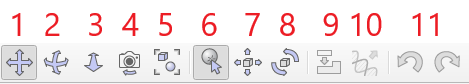
\includegraphics[width=11cm]{toolBar}
\caption{\Large CoppeliaSim 工具列}
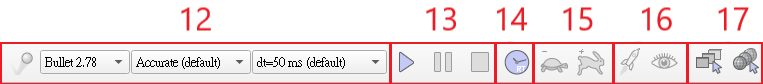
\includegraphics[width=13cm]{toolBar2}
\caption{\Large CoppeliaSim 工具列(續)}
\end{figure}
\begin{table}[hbt!]
\center
\large
\setlength{\tabcolsep}{0.75cm}{
\begin{tabular}{|c|c|c|c|}
\hline  代號 & 功能說明 & 代號 & 功能說明\\
\hline  1 &畫面平移& 10 &複製所有設定\\
\hline  2 &畫面旋轉& 11 &回復/取消回復\\
\hline  3 &畫面縮放&12&模擬設定\\
\hline  4 &畫面視角&13&開始/暫停/停止 模擬\\
\hline  5 &畫面縮放至適當大小&14&即時模擬切換\\
\hline  6 &選取物件&15&模擬速度控制\\
\hline  7 &移動物件&16&線程渲染/視覺化\\
\hline  8 &旋轉物件&17&場景/頁面 選擇\\
\hline  9 &加入/移出 樹狀結構&&\\
\hline 
\end{tabular}}
\caption{\Large 功能說明}
\end{table}
\newpage
%\item 模擬執行\\%
\end{enumerate}
\section{影像處理}

\qquad 在影像處理中我們主要使用了Python套件中的OpenCV(全稱:Open Source Computer Vision Library),並搭配其他套件或模組進行了影像處裡,藉此來取得訓練神經網路訓練時所需的資訊。\\
\begin{figure}[hbt!]
\center

\includegraphics[width=10cm]{pythonCVlogo}
\caption{\Large OpenCV 及Python logo}
\end{figure}

\subsection{CoppeliaSim中的Vision sensor(視覺傳感器)}
\qquad CoppeliaSim的視覺傳感器輸出的影像是以每個像素中以RGB三個位元組所組成的,舉例來說:在CoppeliaSim中視覺傳感器取出畫面像素為512*256,則我們會接收到(512*256)像素*3=393,216個資料,是一筆相當大的資料,所以在影像處理上會消耗掉大量的資源。\\

\subsection{影像辨識}
 透過CoppeliaSim中的Vision sensor接收場景影像並輸出後,便可以開始進行影像辨識的處理。\\
\begin{enumerate}
\item RGB與HSV的轉換\\
RGB即光的三原色Red(紅)Green(綠)Blue(藍),HSV則是一種將RGB色彩模型中的點在圓柱坐標系中的表示法,HSV分別表示Hue(色相)、Saturation(飽和度)、Value(明度),而會將RGB轉換為HSV是因為HSV相較於RGB可以更直接的判斷色彩、明暗和鮮豔度對於顏色過濾可以更方便定義出色彩範圍。\\
\begin{figure}[hbt!]
\center
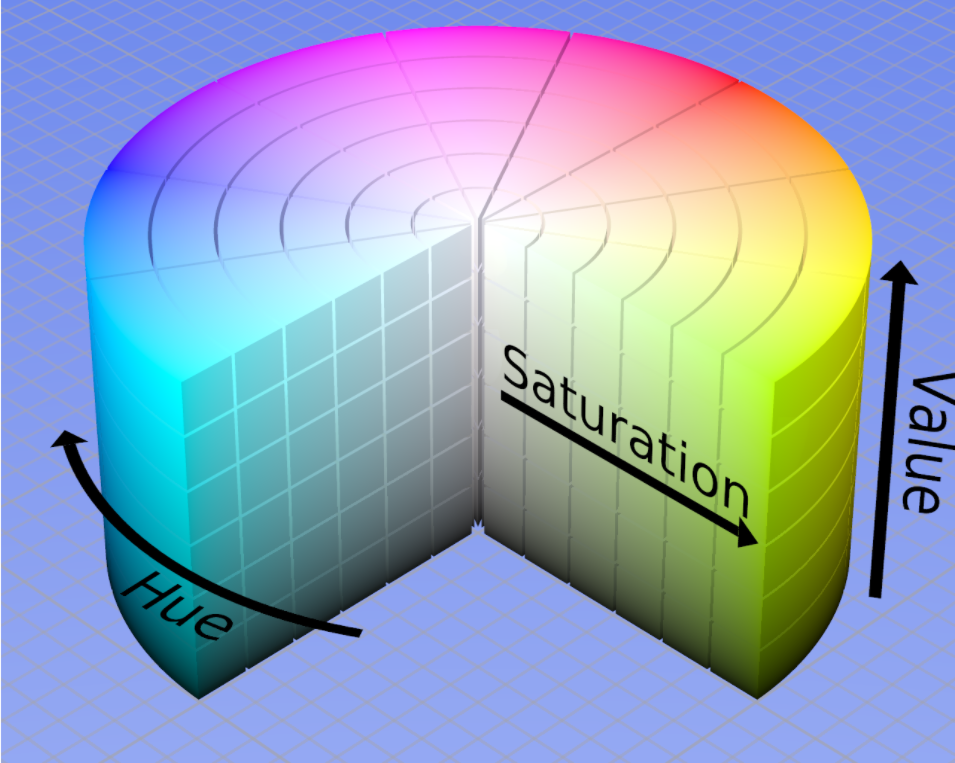
\includegraphics[width=10cm]{HSV}
\caption{\Large HSV色彩空間}
\end{figure}
\newpage
下列為RGB與HSV之間轉換的公式,首先是RGB轉為HSV,其中$max$及$min$分別為$(r,g,b)$中的最大與最小值:
$$h=\left\{\begin{matrix}
0^{\circ}, & \textrm{if}\ max=min\\ 
60^{\circ}+\frac{g-b}{max-min}+0^{\circ},& \textrm{if}\ max=r\;and\;g\geq \;b\\ 
60^{\circ}+\frac{g-b}{max-min}+360^{\circ}, & \textrm{if}\ max=r\;and\;g<  \;b\\ 
60^{\circ}+\frac{g-b}{max-min}+120^{\circ}, & \textrm{if}\ max=g\\ 
60^{\circ}+\frac{g-b}{max-min}+240^{\circ}, & \textrm{if}\ max=b
\end{matrix}\right.$$

$$s=\left\{\begin{matrix}
0, & \textrm{if}\,max=0\\ 
\frac{max-min}{max}=1-\frac{min}{max}, & \textrm{otherwise}
\end{matrix}\right.$$

$$v=max$$
接著是HSV轉為RGB:
$$\textrm{when}\,0\leq H< 360,0\leq S\leq 1,0\leq V\leq 1$$
$$C=V\times S$$
$$X=C\times (1-\left | (H/60^{\circ})\textrm{mod}2-1 \right |)$$
$$m=V-C$$

$$({R}',{G}',{B}')=\left\{\begin{matrix}
(C,X,0)& ,0^{\circ}\leq H< 60^{\circ}\\ 
 (X,C,0)& ,60^{\circ}\leq H< 120^{\circ}\\ 
 (0,C,X)& ,120^{\circ}\leq H< 180^{\circ}\\ 
 (0,X,C)& ,180^{\circ}\leq H< 240^{\circ}\\ 
 (X,0,C)& ,240^{\circ}\leq H< 300^{\circ}\\ 
 (C,0,X)& ,300^{\circ}\leq H< 360^{\circ}
\end{matrix}\right.$$


$$(R,G,B)=(({R}'+m)\times 255,({G}'+m)\times 255,({B}'+m)\times 255)$$

\item 顏色過濾\\
進行顏色過濾時,需要先定義出過濾顏色的上下限,在開始過濾後僅會保留介於上下界線範圍的影像,而介於上下限範圍之外的影像則會被剃除,如圖.\ref{filter}所示以上限(77,255,255)及下限(35,43,46)為例。\\
\begin{figure}[hbt!]
\center
\begin{minipage}[t]{0.48\textwidth}
\center
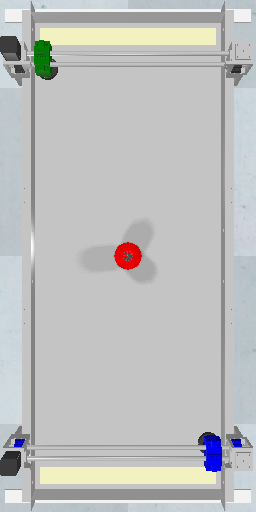
\includegraphics[width=6cm]{origin}
\caption{\Large 場景原圖}
\label{origin}
\end{minipage}
\begin{minipage}[t]{0.48\textwidth}
\center
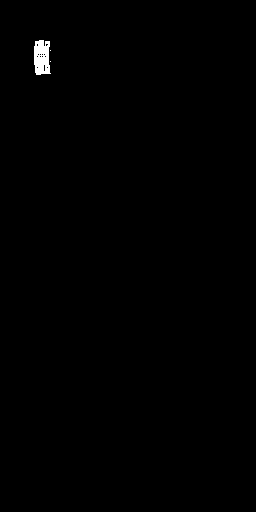
\includegraphics[width=6cm]{filter}
\caption{\Large 顏色過濾後的場景}
\label{filter}
\end{minipage}
\end{figure}


%\item 雜訊去除\\
%為了避免環境因素干擾,使影像產生雜訊並影響了影像辨識度,所以在雜訊的去除也是很重要的,

\end{enumerate}

\newpage